% !TEX TS-program = pdflatex
% !TEX encoding = UTF-8 Unicode

% This is a simple template for a LaTeX document using the "article" class.
% See "book", "report", "letter" for other types of document.

\documentclass[11pt]{article} % use larger type; default would be 10pt

\usepackage[utf8]{inputenc} % set input encoding (not needed with XeLaTeX)

%%% Examples of Article customizations
% These packages are optional, depending whether you want the features they provide.
% See the LaTeX Companion or other references for full information.

%%% PAGE DIMENSIONS
\usepackage{geometry} % to change the page dimensions
\geometry{a4paper} % or letterpaper (US) or a5paper or....
% \geometry{margin=2in} % for example, change the margins to 2 inches all round
% \geometry{landscape} % set up the page for landscape
%   read geometry.pdf for detailed page layout information

\usepackage{graphicx} % support the \includegraphics command and options

% \usepackage[parfill]{parskip} % Activate to begin paragraphs with an empty line rather than an indent

%%% PACKAGES
\usepackage{booktabs} % for much better looking tables
\usepackage{array} % for better arrays (eg matrices) in maths
\usepackage{amsfonts} % for maths fonts
\usepackage{amsmath} % for mathy text templates (propositions, theorems etc.)
\usepackage{amsthm} % proof env
\usepackage[hidelinks]{hyperref} % clickable, interactive references to equations, pages etc
\usepackage{paralist} % very flexible & customisable lists (eg. enumerate/itemize, etc.)
\usepackage{verbatim} % adds environment for commenting out blocks of text & for better verbatim
\usepackage{subfig} % make it possible to include more than one captioned figure/table in a single float
% These packages are all incorporated in the memoir class to one degree or another...

%%% HEADERS & FOOTERS
\usepackage{fancyhdr} % This should be set AFTER setting up the page geometry
\pagestyle{fancy} % options: empty , plain , fancy
\renewcommand{\headrulewidth}{0pt} % customise the layout...
\lhead{}\chead{}\rhead{}
\lfoot{}\cfoot{\thepage}\rfoot{}

%%% SECTION TITLE APPEARANCE
\usepackage{sectsty}
\allsectionsfont{\sffamily\mdseries\upshape} % (See the fntguide.pdf for font help)
% (This matches ConTeXt defaults)

%%% ToC (table of contents) APPEARANCE
\usepackage[nottoc,notlof,notlot]{tocbibind} % Put the bibliography in the ToC
\usepackage[titles,subfigure]{tocloft} % Alter the style of the Table of Contents
\renewcommand{\cftsecfont}{\rmfamily\mdseries\upshape}
\renewcommand{\cftsecpagefont}{\rmfamily\mdseries\upshape} % No bold!

%%% Math templates
\newtheorem{prop}{Proposition}
\newtheorem{lem}{Lemma}
\newtheorem{cor}{Corollary}
\newtheorem{thm}{Theorem}
\newtheorem{defn}{Definition}

%%% END Article customizations

%%% The "real" document content comes below...

\title{An introduction to the mathematics of reinforcement learning theory}
\author{Sebastian Scherer}
%\date{} % Activate to display a given date or no date (if empty),
         % otherwise the current date is printed 

\begin{document}

\maketitle

\section{The agent and the environment}\label{agentEnvironment}

In reinforcement learning we concern ourselves with optimising the behaviour of an agent acting in a given environment. The agent's behaviour is governed by what we call control laws which act on the environment's current state, and can be probabilistic in nature. The environment responds to the agent's actions by assuming a new state. The process of obtaining this new state can also be probabilistic. 

There are some constrains to this very general setting, which we will outline in this section. 

Firstly, we assume that at any time $t \in \mathbb{N}_0$, the environment can only assume one of finite states $s \in S$, where $S$ is the finite set of states possible. 

Similarly, we demand that our agent has only a finite set of actions $a \in A$, where $A$ is the finite set of actions, at his disposal at any given time $t \in \mathbb{N}_0$.

For an arbitrary but fixed starting state $s_0 \in S$, the continuous back-and-forth between the agent choosing an action $a_t$ and the environment assuming a subsequent state $s_{t+1}$ for $t=0,\dots,i$ leads to \textit{state-action trajectories} of the form

\begin{equation}\label{stateActionTraj}
	(s_0, a_0, s_1, a_1, \cdots, s_{i-1},a_{i-1},s_i,a_i).
\end{equation}

We will also sometimes refer to \textit{state trajectories}

\begin{equation}\label{stateActionTraj}
	(s_0, s_1, \cdots, s_{i-1},s_i,)
\end{equation}

 and \textit{action trajectories}

\begin{equation}\label{actionTraj}
	(a_0, a_1, \cdots, a_{i-1},a_i,)
\end{equation}

as needed. For any arbtrarily given but fixed end point in time $i \in \mathbb{N}_0$, we can imbue all of these three trajectory spaces with probability distributions depending on the control laws governing the actions (where plausible), and the probabilistic behaviour of the environment. We will do this in the next section.

Lastly, we require our environment has no memory when evolving from one state to the next, be it in response to our agent's chosen action or otherwise. We demand that the environment's state at time $i+1$, $s_{i+1} \in S$, only depends on the previous time step's state, $s_i \in S$, and the agent's chosen action $a_i \in A$ at time $i$, but \textit{not} on any other preceding states and actions $s_t, a_t, t < i$ forming the state-action trajectory leading up to the state $s_i$ and action $a_i$ at time $i$. To be more precise, we require the \textit{transitional probabilities} of our environment to satisfy

\begin{equation}\label{transProbMarkov}
	Pr(s_{i+1} = s' | (s_0, a_0, \dots, s_i, a_i)) = Pr(s_{i+1} = s' | (s_i,a_i)) =: P^{a_i}_{s_i} (s')
\end{equation}

for all $s' \in S$ and $i \in \mathbb{N}_0$. This property is often referred to as the \textit{Markov} property.

\section{Probabilistic control laws}\label{probControlLaws}

In this section we will formalize our understanding of a \textit{control law}, which can be regarded as the decision making process of our agent at a fixed time $i \mathbb{N}_0$. A control law $\mu$ is a set of probability distributions over the action space $A$, one conditional distribution $\mu(s, \cdot)$ for each possible state $s \in S$. The idea is that, using the control law $\mu$ at time $i$ to make our agent's decision $a_i$, for any possible environment state $s$ $\mu$ generates a probability distribution over the action space $A$, assigning a probability

\begin{equation}\label{controlProb}
	\begin{array}{ll}
			& 	Pr(\text{Choosing action }a_i | \text{The environment is in state } s_i \text{ while following control law }\mu) \\
		=	&	Pr(\text{Choosing action }a_i | s_i, \mu) \\
		=:	&	\mu(s_i, a_i).
	\end{array}
\end{equation}

For completeness, we note that for any such control law $\mu$ clearly 

\begin{equation}\label{controlProbPositive}
	\mu(s,a) \ge 0
\end{equation}

 for every state action pair $(s,a) \in S \times A$, as well as 

\begin{equation}\label{controlProbSum1}
	\sum_{a \in A} \mu(s,a) = 1
\end{equation}

for all $s \in S$, must hold. 

It is worth noting that by the above interpretation we are only allowing control laws and distributions conditioned on \textit{only the immediate state} $s_i$, and nothing else. In this sense, the control laws considered have no memory of past environmental or agent behaviour either.

Before we conclude this section, let us develop a slightly more abstract but, as we shall see later, highly useful perspective on the set of control laws just outlined. We first order the finite state and action sets arbitrarily: $s^1,\dots,s^{|S|}$ and $a^1,\dots,a^{|A|}$. Since any control law $\mu$ is a collection of $|S|$ discrete probability distributions over $A$, we can identify $\mu$ with an element from $\mathbb{R}^{|S| \times |A|}$ via the canonical representation

\begin{equation}\label{controlProbMatrix}
	\mu = \left(	\begin{array}{cccc}
					\mu(s^1,a^1)	&	\mu(s^1,a^2)	&	\cdots 	&	\mu(s^1,a^{|A|}) \\
					\mu(s^2,a^1)	&	\mu(s^2,a^2)	&	\cdots 	&	\mu(s^2,a^{|A|}) \\
					\vdots 		&	\vdots 		& 	\ddots 	& 	\vdots \\
					\mu(s^{|S|},a^1)	&	\mu(s^{|S|},a^2)	&	\cdots 	&	\mu(s^{|S|},a^{|A|}) \\
				\end{array}
		\right).
\end{equation}

Here, the $i$-th row of the right hand side encodes the conditional probability distribution $\mu(s^i, \cdot)$ conditioned on state $s^i \in S$. We can thus see that the set of control laws can be identified with a closed and bounded, and therefore \textit{compact}, subset of the $\mathbb{R}^{|S| \times |A|}$ with its canonical norm via

\begin{equation}
	\Big\{ \mu | \mu \text{ is a control law} \Big\} = \Big\{ \mu \in \mathbb{R}^{|S| \times |A|} \Big| \mu_{ij} \ge 0 \, \forall i,j, \, \sum_{j=1}^{|A|} \mu_{ij} = 1 \, \forall i=1,\dots,|S| \Big\}.
\end{equation}

The identification of the set of control laws with a compact set will be crucial in maximization arguments further down the line. Before that, however, let us next see how we can use these control laws to formalize the behaviour of our agent.

\section{Control law sequences and state-action trajectories}\label{controlLawTrajs}

In the previous section we have formalized the nature of our agent's decision making process at any given time $i$: Given that the environment is in state $s_i$ and our agent follows the control law $\mu$, it will pick any action $a \in A$ with probability $\mu(s_i,a)$. There is no reason for us to constrain our agent to keep using the same control law $\mu$ over time. It is much more desirable for our agent to be able to follow a sequence of different control laws, say,

\begin{equation}\label{controlLawSeqence}
	\vec{\mu}(i) = (\mu_0, \mu_1, \dots, \mu_i),
\end{equation}

where $\mu_t$ is the control law employed at time $t = 0,\dots i$ by our agent to pick action $a_i$. As referred to earlier, an environment with known transition probabilities $P^a_{ss'}, a \in A, s,s' \in S$ together with a sequence $\vec{\mu}(i)$ of control laws of length $i$ induces probability distributions on the sets of state-action, state and action trajectories. The environment's Markov property and the control laws' lack of memory allow for a nice factorization of these probabilities. The following Lemma makes this claim more precise.

\begin{figure}
  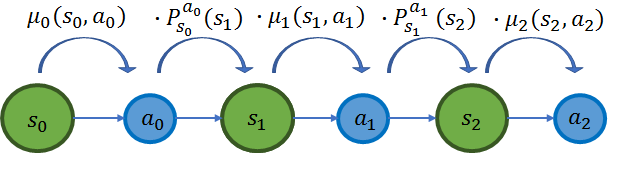
\includegraphics[width=\linewidth]{../graphics/state_action_probs.png}
  \caption{A trajectory starting from $s_0$ while following $\mu_0,\dots,\mu_i$ for $i = 2$}
  \label{fig:boat1}
\end{figure}

\begin{lem}{(State-action trajectory distribution under policies)}\label{lemStateActionControlLawTrajProb}

For some $i \in \mathbb{N}_0$, let $\vec{\mu}(i)$ be a finite series of probabilistic control laws. Then for any fixed starting state $s_0 \in S$ and state-action trajectory $(s_0,a_0,\dots,s_i,a_i)$, the probability of obtaining said state-action trajectory up to time $i$ while following $\vec{\mu}(i)$ is given by

\begin{equation}\label{stateActionControlLawTrajProb1}
	\prod_{t=0}^{i-1} \left( \mu_t(s_t,a_t) \cdot P^{a_t}_{s_t}(s_{t+1}) \right) \cdot \mu_i(s_i,a_i).
\end{equation}

\end{lem}

\begin{proof}

We prove this claim via induction over the control law sequence length parameter $i$. Since $i=0$ is somewhat trivial, we start our induction with $i=1$. We see that

\begin{equation}\label{controlLawTrajIA}
	\begin{array}{ll}
			& \Pr\{(s_0,a_0, s_1, a_1) | \text{ starting at } s_0 \text{ and following } \vec{\mu}(1) = (\mu_0,\mu_1)\} \\
		=	& \Pr\{(s_0,a_0, s_1, a_1) | s_0, \, \vec{\mu}(1)\} = \Pr\{(s_0,a_0) \cap (s_1,a_1) | s_0, \, \vec{\mu}(1)\} \\
		=	& \Pr\{(s_0,a_0, s_1) | s_0, \, \vec{\mu}(1)\} \cdot \Pr\{a_1 |(s_0,a_0,s_1), \, s_0, \, \vec{\mu}(1)\} \\
		=	& \Pr\{(s_0,a_0,s_1) | s_0, \, \mu_0\} \cdot \Pr\{a_1 | s_1, \, \mu_1)\} \\
		=	& \Pr\{(s_0,a_0) | s_0, \, \mu_0\} \cdot \Pr\{s_1 | (s_0,a_0), \, \mu_0 \} \cdot \Pr\{a_1 | s_1, \, \mu_1)\} \\
		=	& \mu_0(s_0,a_0) \cdot \, P^{a_0}_{s_0}(s_1) \cdot \mu_1(s_1,a_1). \\
	\end{array}
\end{equation}

Now assume this claim holds for some $i-1 \in \mathbb{N}_0$. The exact same argument applied above then yields

\begin{equation}\label{controlLawTrajIS}
	\begin{array}{ll}
			& \Pr\{(s_0,a_0,\dots, s_i, a_i) | \text{ starting at } s_0 \text{ and following } \vec{\mu}(i)\} \\
		=	& \Pr\{(s_0,a_0,\dots, s_i, a_i) | s_0, \, \vec{\mu}(i)\} \\
		=	& \Pr\{(s_0,a_0,\dots, s_{i-1}, a_{i-1}) \cap (s_i,a_i) | s_0, \, \vec{\mu}(i)\} \\
		=	& \Pr\{(s_0,a_0,\dots, s_{i-1}, a_{i-1},s_i) | s_0, \, \vec{\mu}(i)\} \cdot \Pr\{a_i |(s_0,a_0,\dots, s_{i-1}, a_{i-1},s_i), \, s_0, \, \vec{\mu}(i)\} \\
		=	& \Pr\{(s_0,a_0,\dots, s_{i-1}, a_{i-1},s_i) | s_0, \, \vec{\mu}(i-1)\} \cdot \Pr\{a_i | s_i, \, \mu_i)\} \\
		=	& \Pr\{(s_0,a_0,\dots, s_{i-1}, a_{i-1}) | s_0, \, \vec{\mu}(i-1)\} \\
			& \cdot \Pr\{s_i | (s_0,a_0,\dots, s_{i-1}, a_{i-1}), \, s_0, \, \vec{\mu}(i-1) \} \cdot \Pr\{a_i | s_i, \, \mu_i)\} \\
		=	& \Pr\{(s_0,a_0,\dots, s_{i-1}, a_{i-1}) | s_0, \, \vec{\mu}(i-1)\} \\
			& \cdot \Pr\{s_i | (s_{i-1}, a_{i-1}) \} \cdot \Pr\{a_i | s_i, \, \mu_i)\} \\
		=	& \Pr\{(s_0,a_0,\dots, s_{i-1}, a_{i-1}) | s_0, \, \vec{\mu}(i-1)\} \cdot P^{a_{i-1}}_{s_{i-1}}(s_i) \cdot \mu_i(s_i,a_i) \\
		=	& \prod_{t=0}^{i-2} \left( \mu_t(s_t,a_t) \cdot P^{a_t}_{s_t}(s_{t+1}) \right) \cdot \mu_{i-1}(s_{i-1,}a_{i-1}) \cdot P^{a_{i-1}}_{s_{i-1}}(s_i) \cdot \mu_i(s_i,a_i) \\		
		=	& \prod_{t=0}^{i-1} \left( \mu_t(s_t,a_t) \cdot P^{a_t}_{s_t}(s_{t+1}) \right) \cdot \mu_i(s_i,a_i).
	\end{array}
\end{equation}

\end{proof}

Similarly, without executing the last action at time $t = i$ and thus effectively only following $\vec{\mu}(i-1) = (\mu_0,\dots,\mu_{i-1})$ we obtain the corollary result

\begin{cor}(State-action trajectory distribution under policies II)\label{corStateActionControlLawTrajProb1}

For some $i \in \mathbb{N}_0$, let $\vec{\mu}(i-1)$ be a finite series of probabilistic control laws. Then for any fixed starting state $s_0 \in S$ and state-action trajectory $(s_0,a_0,\dots,s_i)$, the probability of obtaining said state-action trajectory up to time $i-1$ while following $\vec{\mu}(i-1)$ is given by

\begin{equation}\label{stateActionControlLawTrajProb2}
	\prod_{t=0}^{i-1} \left( \mu_t(s_t,a_t) \cdot P^{a_t}_{s_t}(s_{t+1}) \right).
\end{equation}

\end{cor}

Given a some starting state $s_0$, what about the chances of following \textit{any} state-action trajectory ending with some specified state-action pair $(s_i,a_i) \in S \times A$? Clearly, the answer is to simply add over all relevant state-action trajectory probabilities.

\begin{cor}(State-action trajectory distribution under policies III)\label{corStateActionControlLawTrajProb2}

For some $i \in \mathbb{N}_0$, let $\vec{\mu}(i)$ be a finite series of probabilistic control laws, and let $(s,a) \in S \times A$ be any fixed but arbitrary state-action pair.Let finally $s_0 \in S$ be some fixed but arbitrary starting state. Then the probability of following \textit{any} of the state-action trajectories $(s_0,a_0,...,s,a)$, $a_t \in A$ for $t=0,...,i-1$, $s_t \in S$ for $t=1,...,i-1$, while following $\vec{\mu}(i)$ is given by

\begin{equation}\label{stateActionControlLawTrajProb3}
	\sum_{\begin{array}{c}
			a_0,\dots,a_{i-1} \in A \\
			s_1,\dots,s_{i-1} \in S
		\end{array}}\Big[ \prod_{t=0}^{i-2} \left( \mu_t(s_t,a_t) \cdot P^{a_t}_{s_t}(s_{t+1}) \right) \cdot \mu_{i-1}(s_{i-1},a_{i-1}) \cdot P^{a_{i-1}}_{s_{i-1}}(s) \Big] \cdot \mu_i(s,a).
\end{equation}

\end{cor}

\begin{proof}

Using Lemma \ref{lemStateActionControlLawTrajProb}, we immediately arrive at the expression in Eq. \ref{stateActionControlLawTrajProb3} by summing over the set of relevant trajectories.

\begin{equation}\label{}
	Tr_{s_0}^{s,a} =  \left\{(s',a_0,s_1,a_1,\dots,s_{i-1},a_{i-1},s,a) \Bigg| \begin{array}{lr}
															a_0, \dots, a_{i-1} \in A, \\
															s' = s_0, \\
															s_1,\dots,s_{i-1} \in S
													\end{array} \right\}.
\end{equation}

\end{proof}

\begin{figure}
  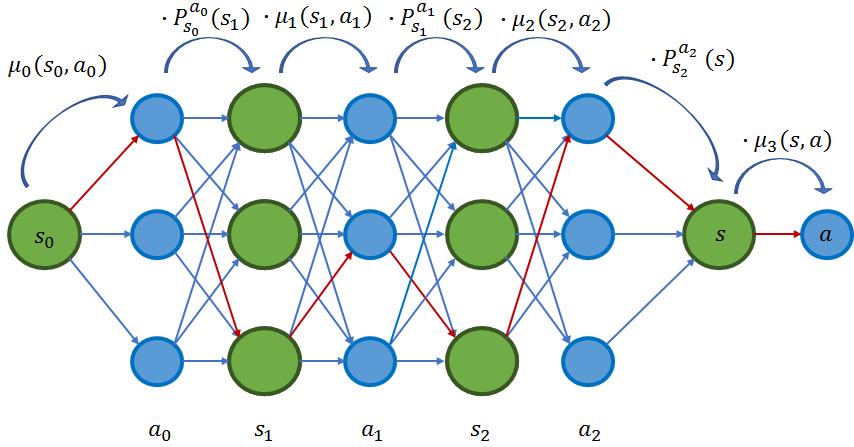
\includegraphics[width=\linewidth,height=7cm]{../graphics/state_action_probs_2.png}
  \caption{All the possible trajectories $(s_0,\dots,s,a)$ starting from $s_0$ while following $\mu_0,\dots,\mu_i$ for $i = 3$, $|S| = |A| = 3$. A sample trajectory is highlighted in magenta.}
  \label{fig:boat1}
\end{figure}

\end{document}